\section{Application Overview}
\label{sec:appOver}


\subsection{Users}
A non-technical user should be able to use this to get meaningful outputs and visualizations. The target audience is a government official or someone in the private sector - it should be clear to them how to get value out of this and what that value is.

\subsection{Architecture}

Figure \ref{fig:archi} shows the architecture of the proposed solution including the elements of the application at component level and its connections at high level (see deployment diagram). Additionally, it shows the application elements used for the Front and Back End. The figure also shows the names of the technologies used hosted on AWS cloud, i.e.: (Python, dash and libraries).   

The following is the list AWS components used in the projec: 
\begin{enumerate}
\item The machine who host the solution (Elastic Compute Cloud - EC2). 
\item The Database  (Relational Database Service -RDS).
\item The storage for the datasets and GeoJson files for Colombia on the service  (Simple Storage Service - S3) to save these files.
\item The Security group for these services talks with each other and have access from the internet as well.
\item The remote DNS (Domain Name Service) to have a friendly URL for the application on the Apache Web server.
\item A remote code repository (hosted by github). It is used for hosting the source code and documentation. 

\end{enumerate}


\begin{figure}%
\centering
\subfigure[Deployment diagram]{%
\label{fig:first}%
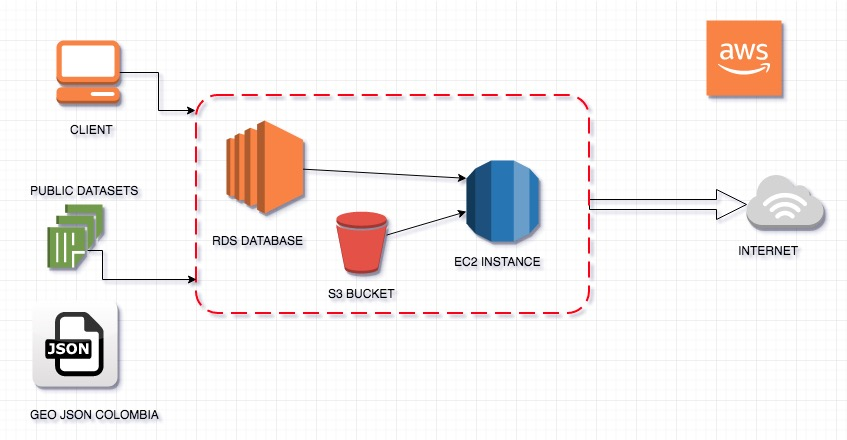
\includegraphics[height=3in, width=4.5in]{../../../aws_diagrams/AWS_Deployment_Diagram_project_group_03}}%
\qquad
\subfigure[Component diagram]{%
\label{fig:second}%
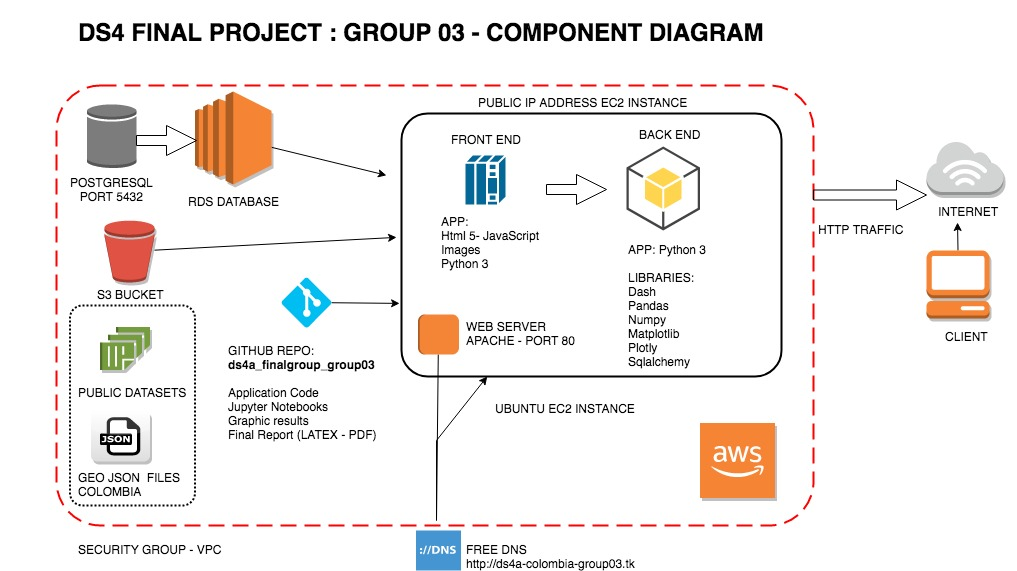
\includegraphics[height=4in, width=6in]{../../../aws_diagrams/AWS_Component_Diagram_project_group_03}}%
\caption{Project architecture.}
\label{fig:archi}%
\end{figure}





\subsection{Front End Design}

The following is the link of the web-page created for the project.
\begin{itemize}
\item \url{http://ds4a-colombia-group03.tk/}
\end{itemize}

Figure \ref{fig:muckup} shows the muckup of the project. In general terms our information system will provide a dynamic map of Colombia delivering:
\begin{enumerate}
\item The impact metric (or metrics) at the municipal level for a given category of events. Ability to display complementary metrics of interest for specific locations (utilities, healthcare facilities, first-responder facilities, etc).
\item Considering the established association between extreme temperatures and the frequency of hydro-meteorological events, a projected extreme-temperature indicator for the 100 most vulnerable municipalities with 3 data points: Indicator value at Time 0 (1998), Time 1 (2018) and Time 3 (projected 2040)
\item The indicator corresponds to the extreme temperature projection made by Climate Impact Lab for the number of days a year that register temperatures above 32 degrees Celsius.
\end{enumerate}

\begin{figure}%
\centering
\subfigure[]{%
\label{fig:first}%
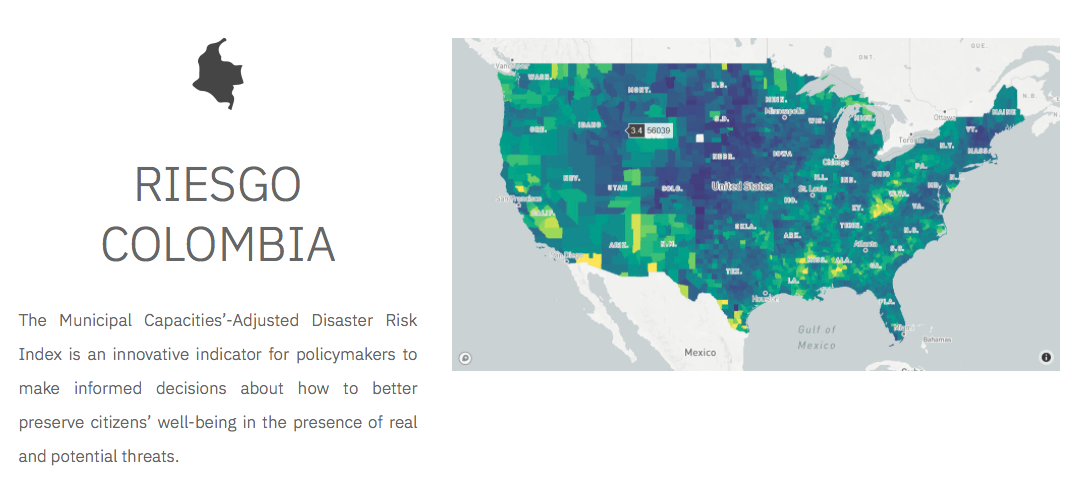
\includegraphics[height=3in, width=6in]{riesgo3}}%
\qquad
\subfigure[]{%
\label{fig:second}%
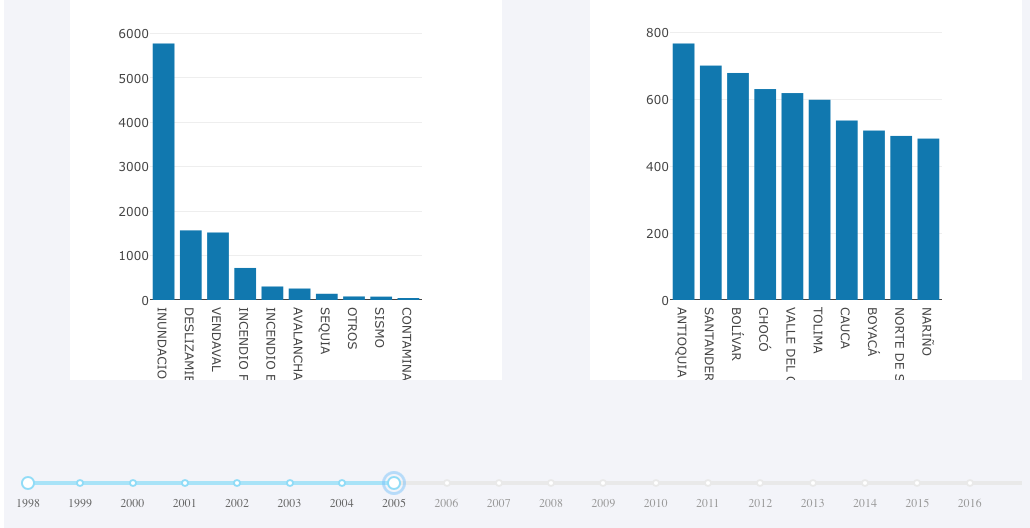
\includegraphics[height=2in, width=3in]{riesgo2}}%
\subfigure[]{%
\label{fig:second}%
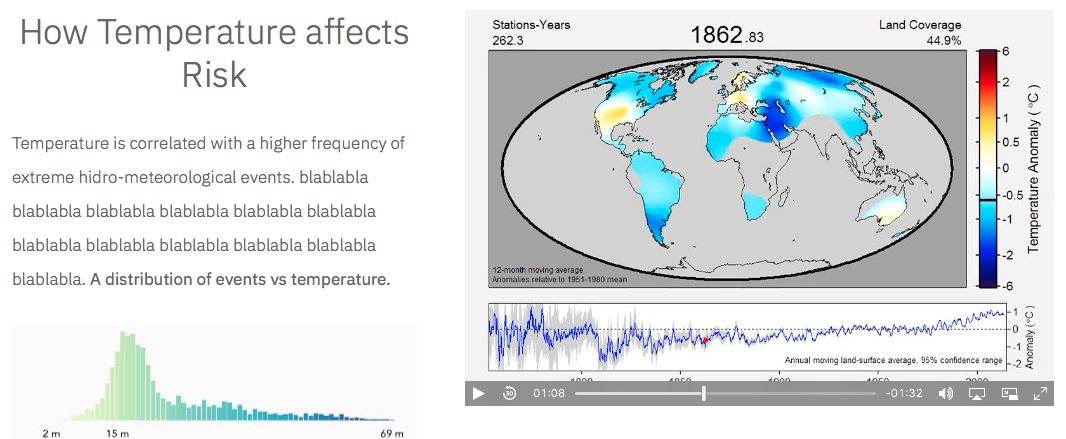
\includegraphics[height=2in, width=3in]{riesgo6}}%
\caption{Muckup of the Hydro-meteorological Risks In Colombia project. The main page (Figure \ref{fig:first}) will show the map of Colombia with the Risk Index, and will offer interactive options to get detail information of selected Municipalities. The page will provide the current risk index in addition to a line plot that shows a projected temperature indicator.}
\label{fig:muckup}%
\end{figure}





\itemize{
\item{Outline of who the primary users would be and how they would interact with the app}
\item{Descriptions of app features}
\item{The datasets your team is planning on using}
\item{How you plan on using each of these datasets/how they contribute to your app}
}